% ISTRUZIONI PER INTEGRARE LE FIGURE NEL CAPITOLO 3
% ================================================

% Aggiungere nel preambolo del documento principale:
\usepackage{graphicx}
\graphicspath{{./figure/}}

% Per includere le figure nel capitolo, sostituire i placeholder con:

% Figura 3.1 - Architettura Edge-Cloud (riga ~86)
\begin{figure}[htbp]
\centering
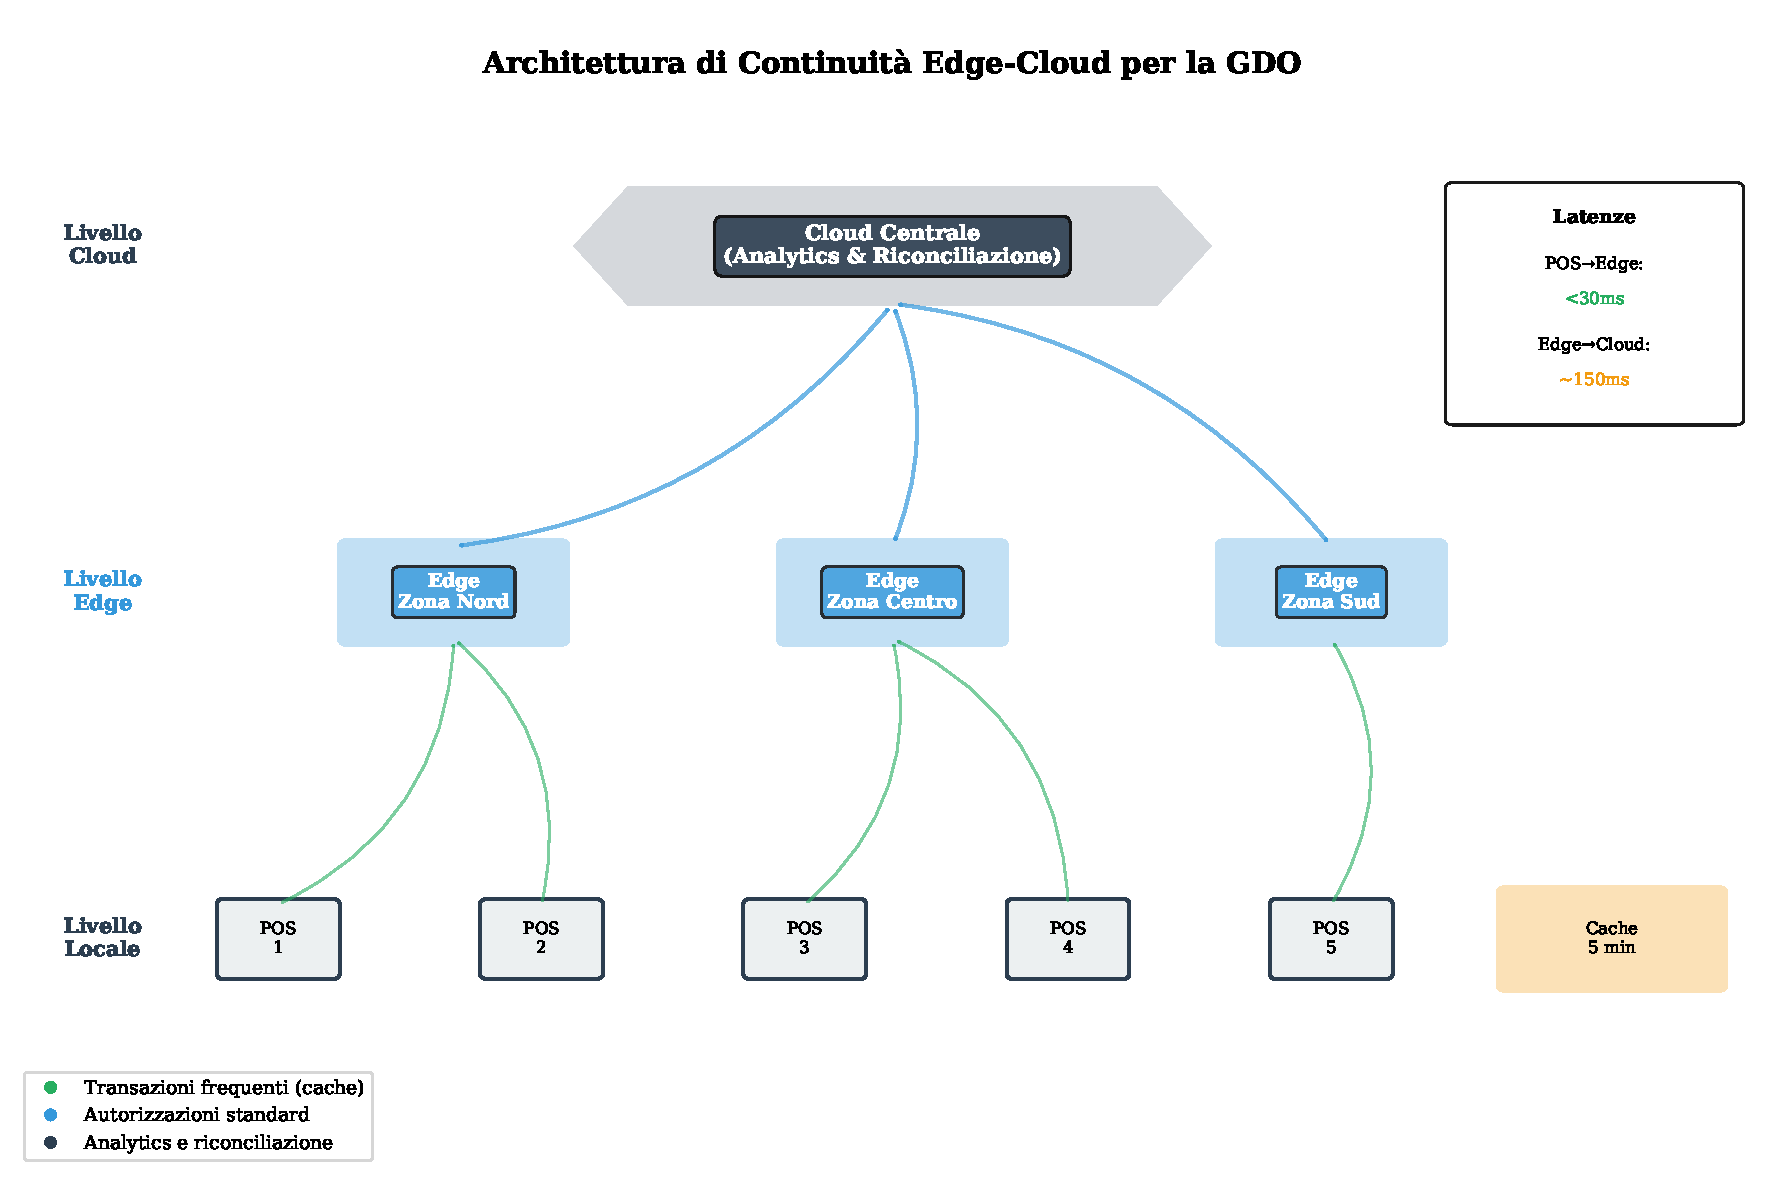
\includegraphics[width=0.9\textwidth]{fig_3_1_edge_cloud_architecture.pdf}
\caption{Architettura di continuità Edge-Cloud per la GDO}
\label{fig:edge-cloud}
\end{figure}

% Figura 3.2 - Multi-Cloud (dopo sezione 3.3.2, ~riga 137)
\begin{figure}[htbp]
\centering
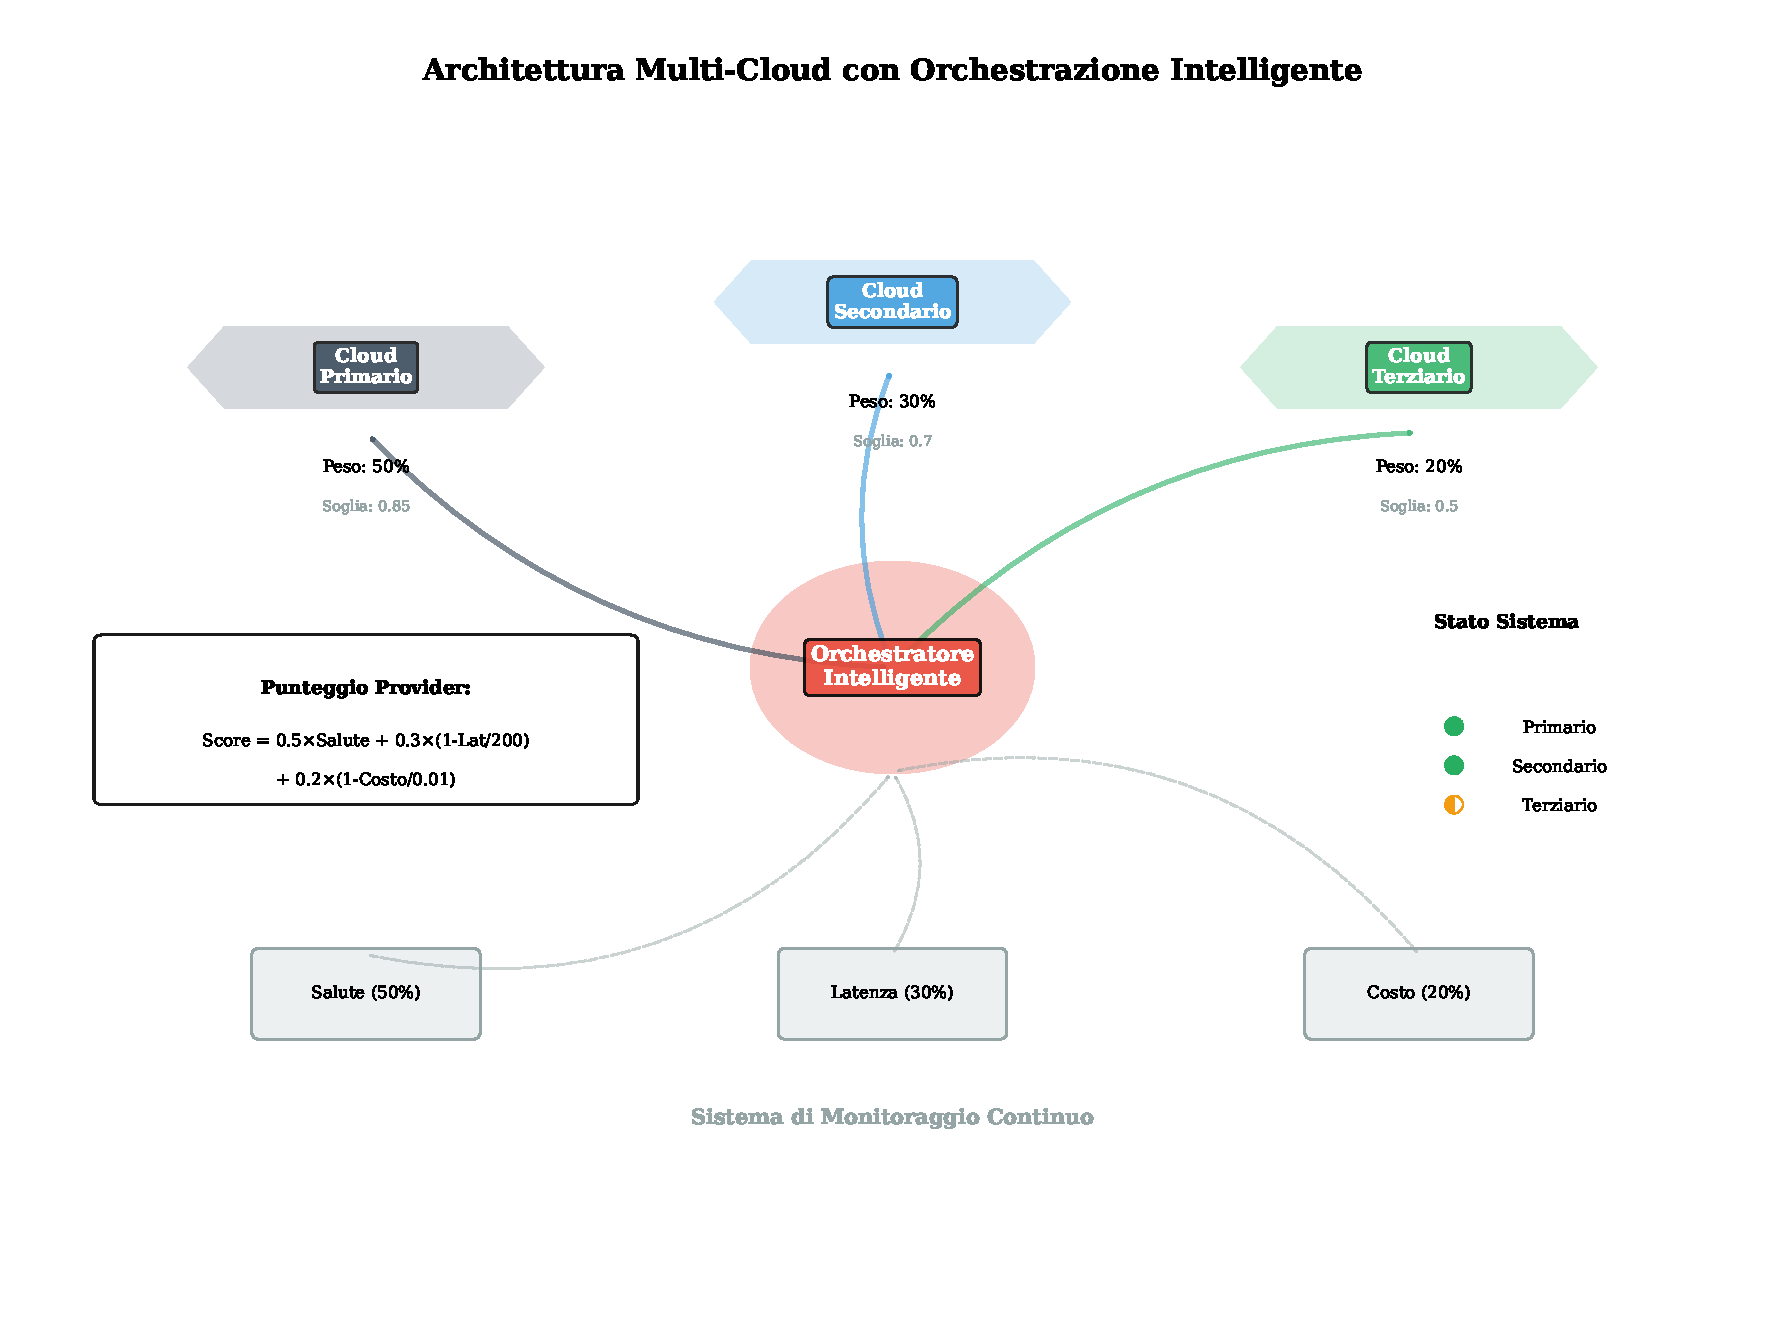
\includegraphics[width=0.9\textwidth]{fig_3_2_multi_cloud.pdf}
\caption{Architettura Multi-Cloud con orchestrazione intelligente per resilienza operativa}
\label{fig:multi-cloud}
\end{figure}

% Figura 3.3 - Compliance-by-Design (dopo sezione 3.3.3, ~riga 150)
\begin{figure}[htbp]
\centering
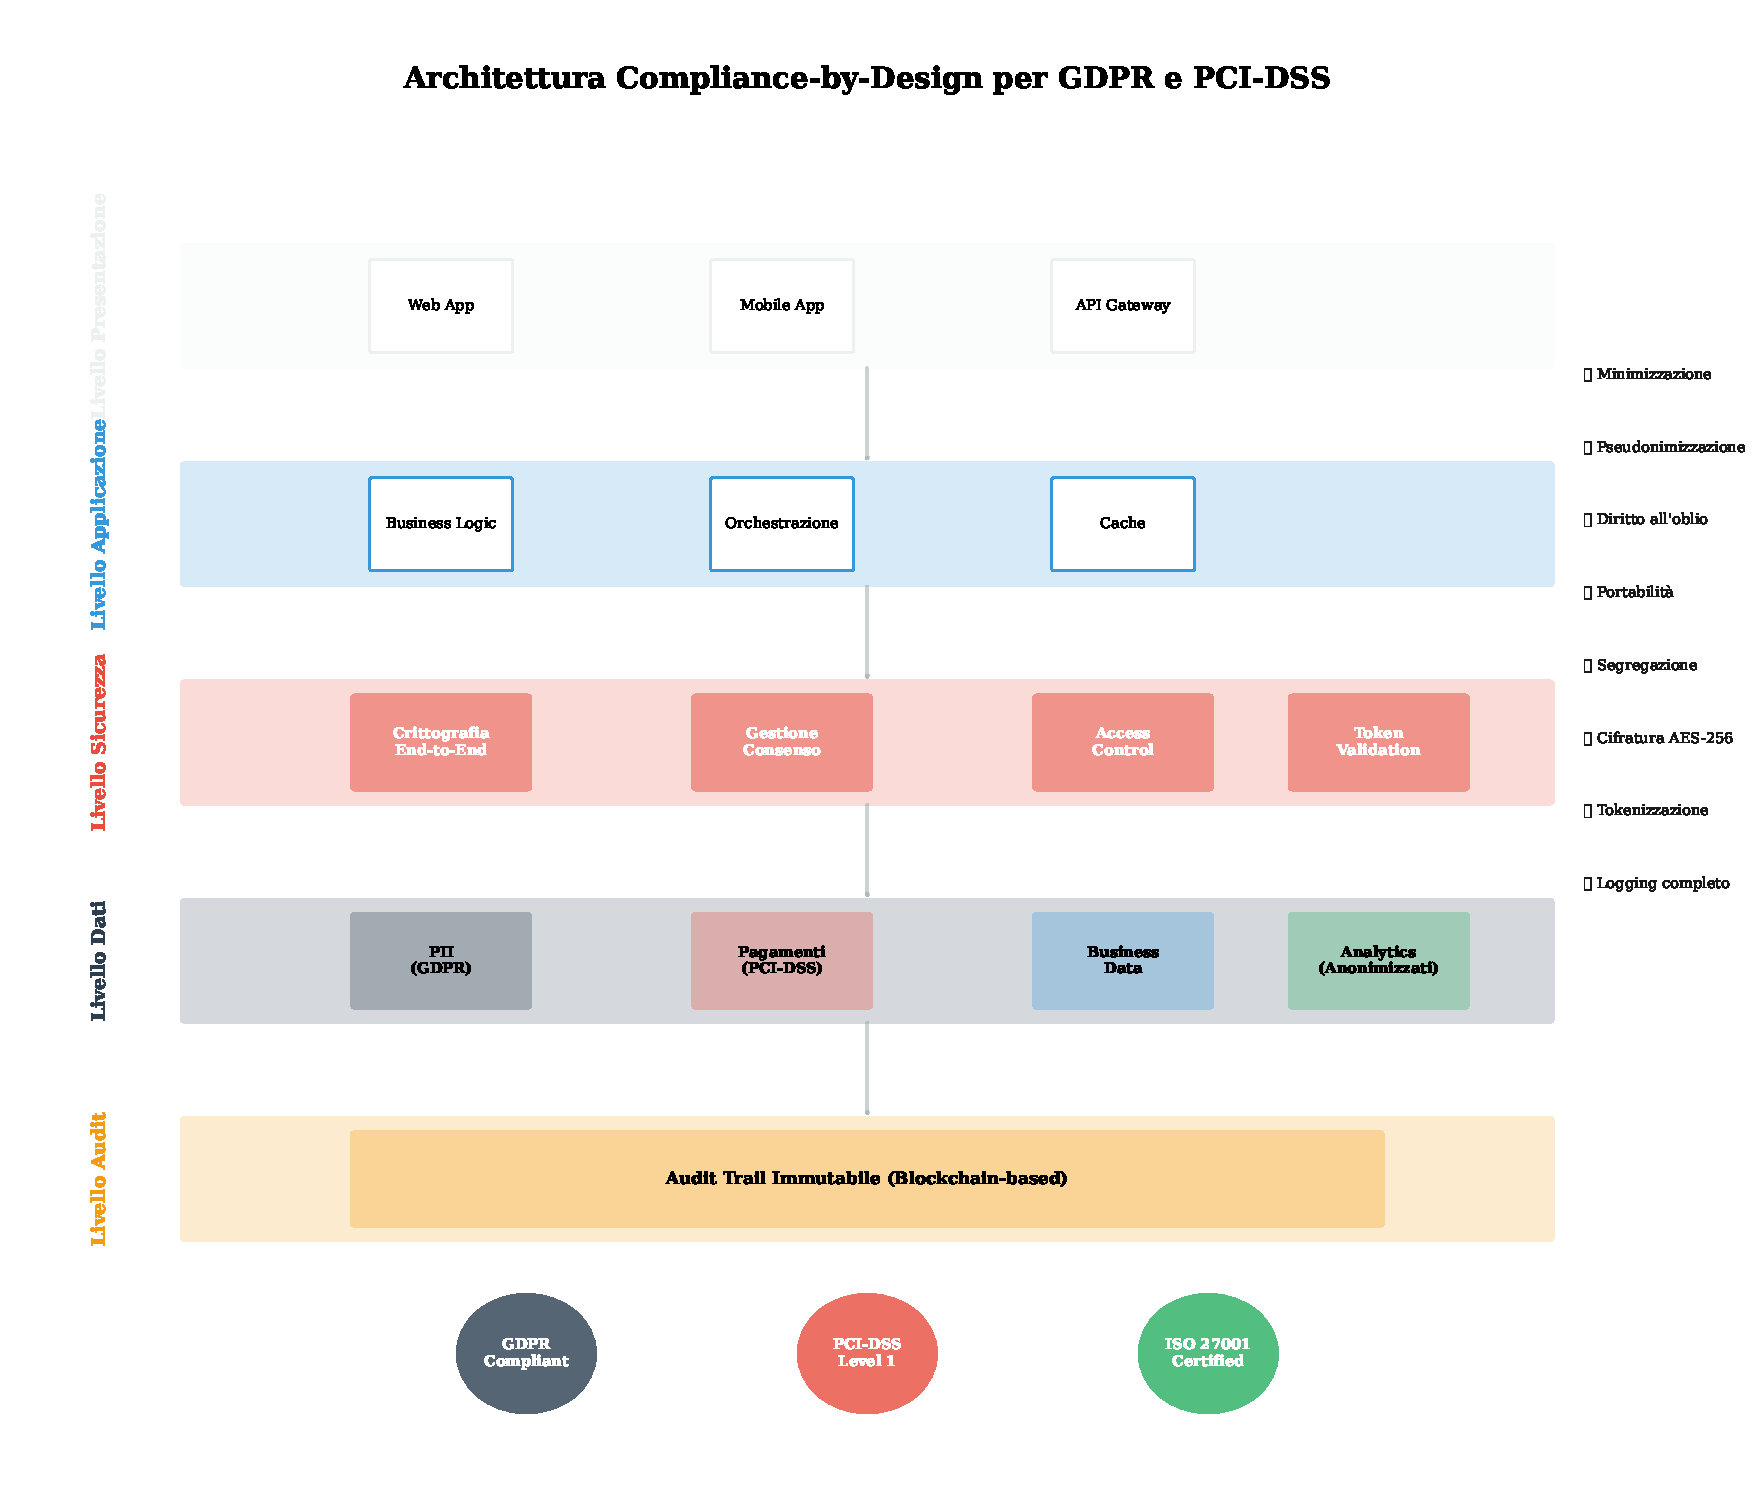
\includegraphics[width=0.9\textwidth]{fig_3_3_compliance_by_design.pdf}
\caption{Architettura Compliance-by-Design con segregazione automatica e audit immutabile}
\label{fig:compliance-design}
\end{figure}

% Figura 3.4 - Sistema di Simulazione (dopo sezione 3.4.1, ~riga 158)
\begin{figure}[htbp]
\centering
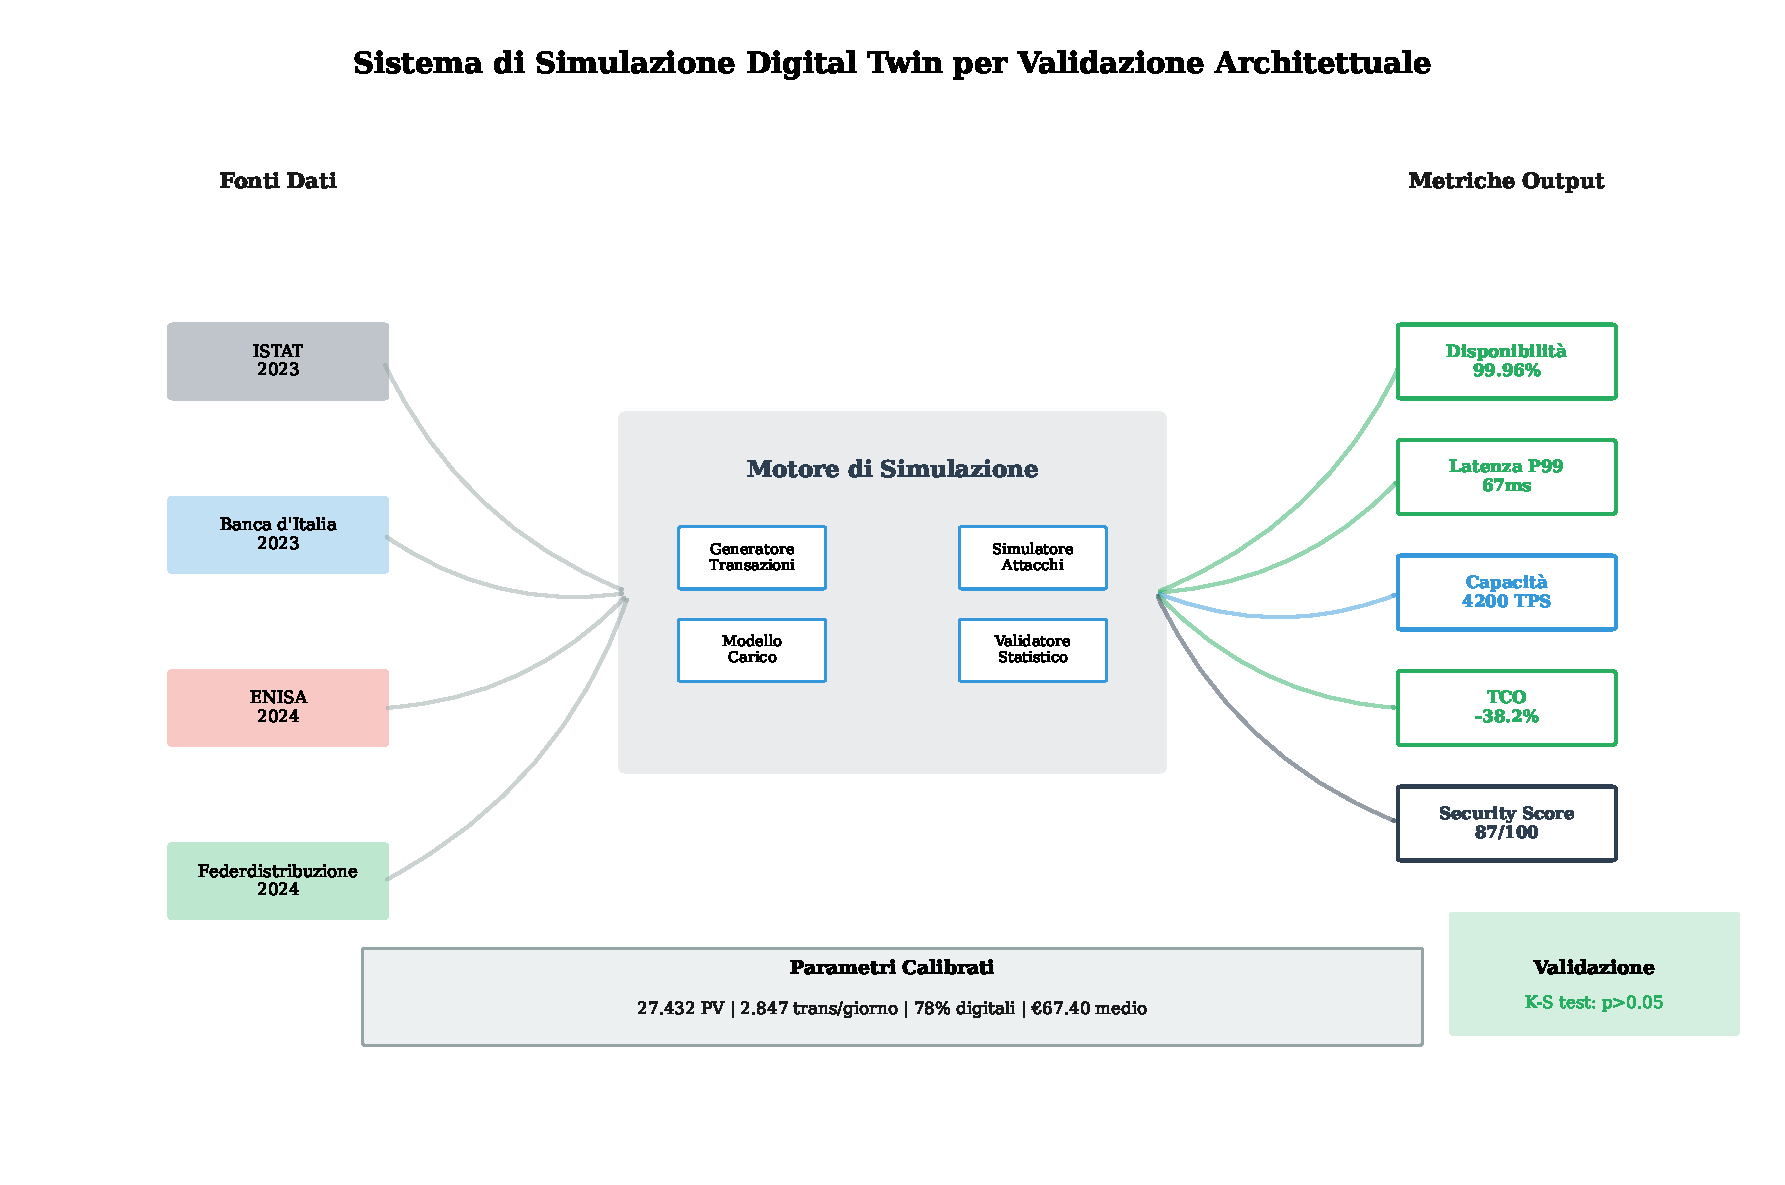
\includegraphics[width=0.85\textwidth]{fig_3_4_simulation_system.pdf}
\caption{Sistema di simulazione Digital Twin per validazione architettuale}
\label{fig:simulation-system}
\end{figure}

% Figura 3.5 - Timeline Migrazione (dopo sezione 3.5.1, ~riga 232)
\begin{figure}[htbp]
\centering
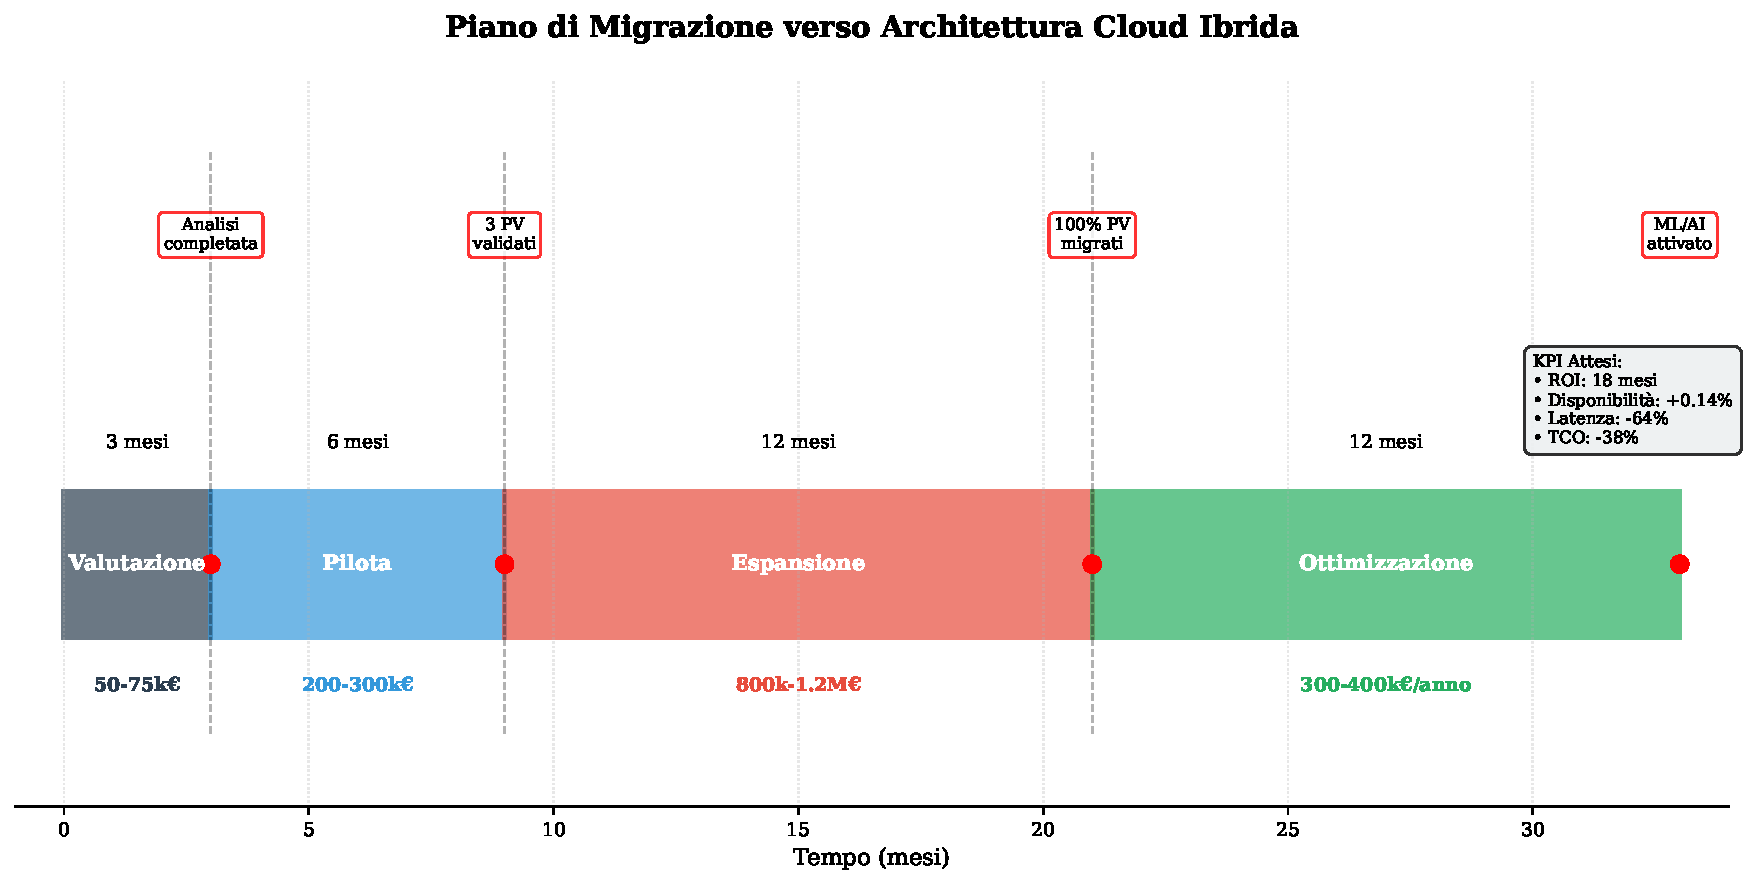
\includegraphics[width=\textwidth]{fig_3_5_migration_timeline.pdf}
\caption{Piano temporale di migrazione verso architettura cloud ibrida}
\label{fig:migration-timeline}
\end{figure}

% Figura 3.6 - Confronto Prestazioni (dopo tabella 3.6, ~riga 208)
\begin{figure}[htbp]
\centering
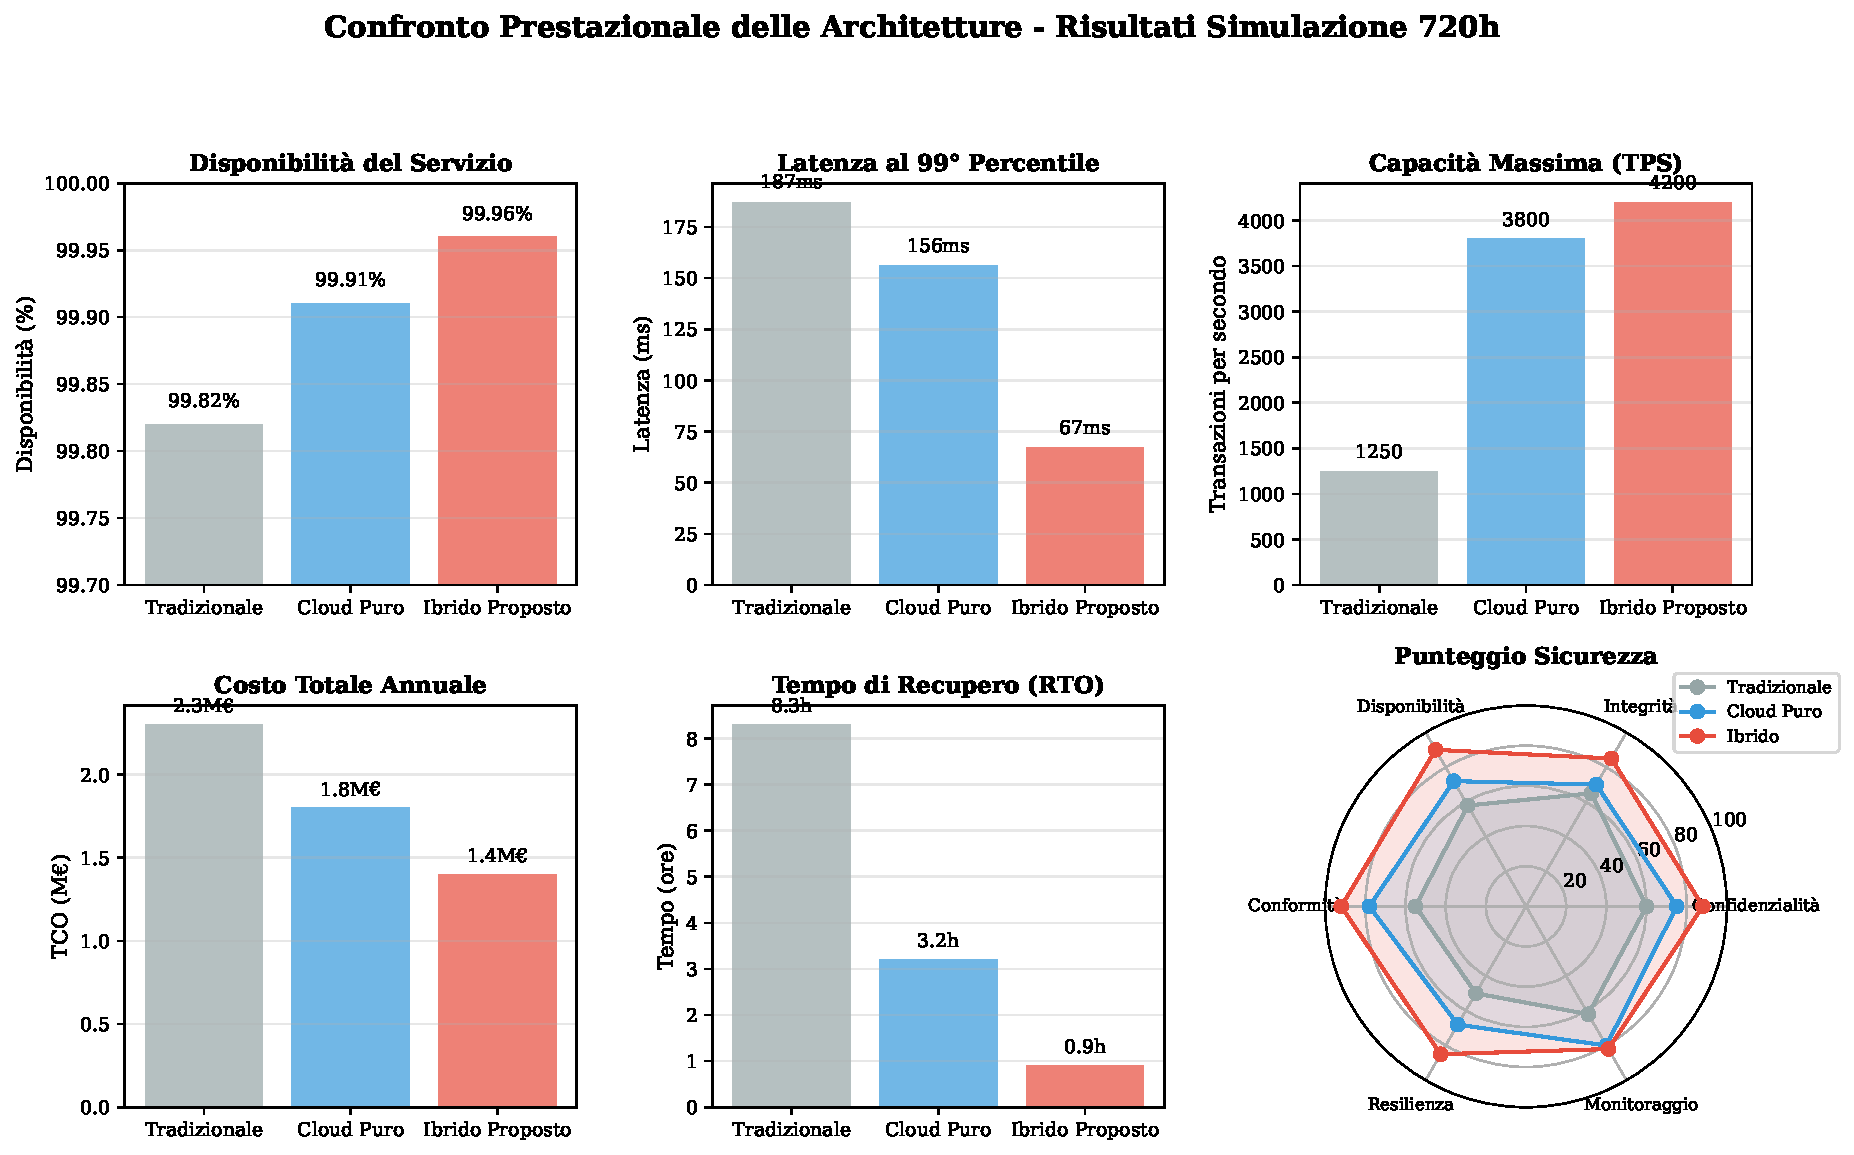
\includegraphics[width=\textwidth]{fig_3_6_performance_comparison.pdf}
\caption{Confronto prestazionale delle architetture attraverso metriche chiave}
\label{fig:performance-comparison}
\end{figure}
